\chapter{Research Problem} \label{chap:research_problem}

In this chapter, we present how the Continuous Integration System of the R\&D IPK team in Synopsys Porto is arranged and what needs to be improved. 

We will describe its architecture in section~\ref{sec:res_system}, with a little description of its different communication interfaces in section~\ref{sec:interfaces} and current continuous integration flow in section~\ref{sc:workflow}. It is also listed the requirements we will implement in the solution in section~\ref{sc:requirements}, following by the current method of displaying the project builds information in section~\ref{sec:spreadsheet}.
Finally a conclusion in section~\ref{sec:conclusion_3} about the problem in study.

\section{The System architecture}\label{sec:res_system}

Most compliance tests take long periods to finish (aprox. 4 hours, as displayed in the figure~\ref{fig:buildView} top-right corner). In addition to setting up and recreating the test environment for each run, it is felt as a waste of time. The current test automation environment, due to its manual labor has some issues such as the inconsistency between tests and the lack of traceability among product versions in testing. Hereupon, we want to increase efficiency and productivity of the R\&D teams in HW/SW testing and improve reporting to these teams.

To this goal, it is desirable to create an automated test architecture that eliminates the need of employing an engineer to configure the equipment by using automated test equipment, which will allow the continuous testing of different features configurations through automation. By consequence this permits an improved and robust test coverage, as well as increasing their number and velocity. This will summarize in a more refined and consistent testing process, with an improved degree of trust and certainty on the results.

This architecture should meet the following requirements:

\begin{itemize}
\item Speed up testing to allow for accelerated releases which:
	\begin{itemize}
		\item Reduces testing costs;
        \item Reduces time in testing phase.
	\end{itemize}
\item Allow testing IP's features continuously;
\item Improve test coverage;
\item Ensure consistency;
\item Improve the reliability of testing;
	\begin{itemize}
		\item Consolidate the testing process
	\end{itemize}
\end{itemize}

  \begin{figure}[H]
  \centering
      \makebox[\textwidth][c]{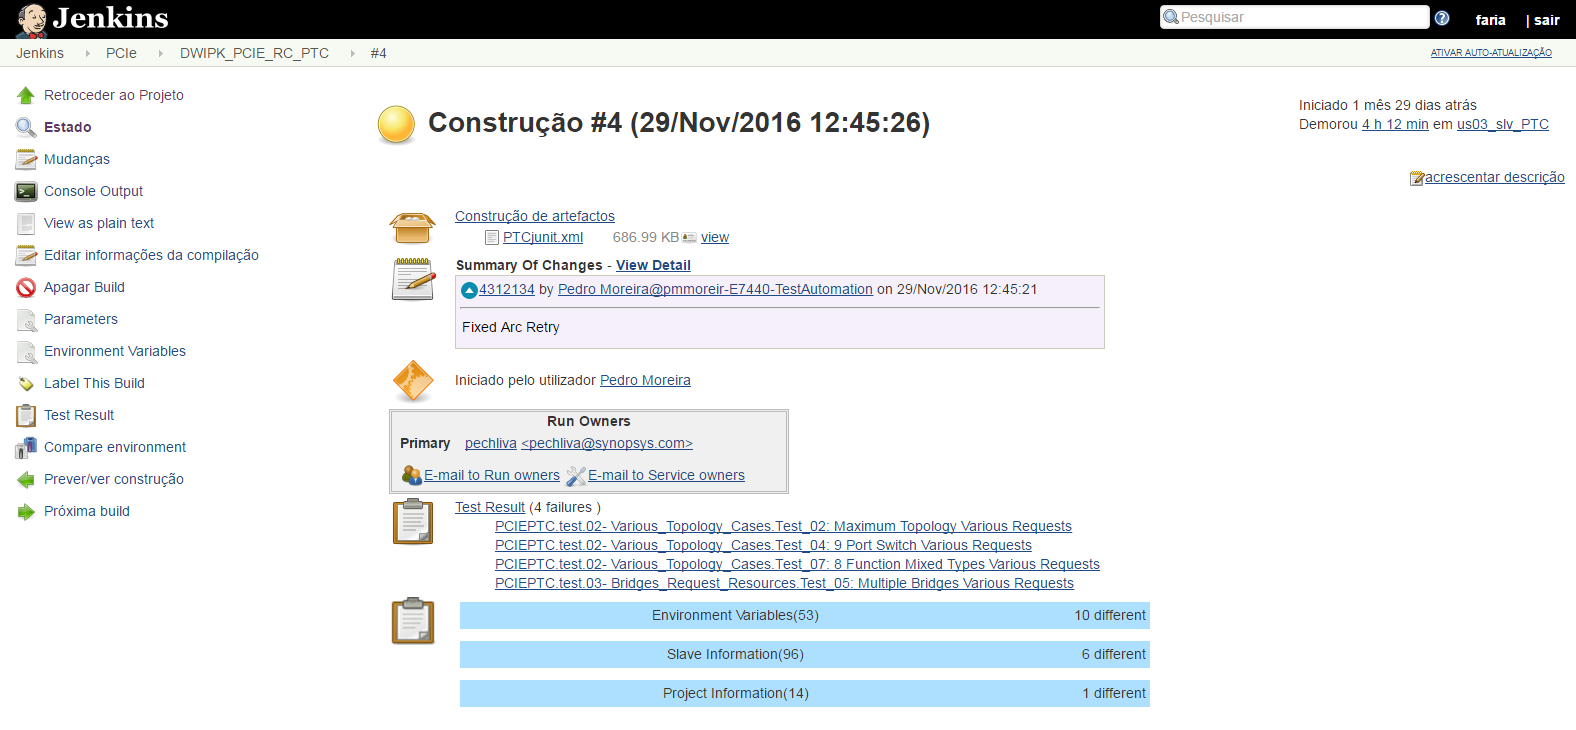
\includegraphics[width=1\textwidth]{buildViewInfo}}
      \caption{View of an example Build}
      \label{fig:buildView}
  \end{figure}

The block diagram shown in the figure~\ref{fig:ci_hw_context} shows the hardware testing architecture which is analogous to a common continuous integration software development setup.

\clearpage

  \begin{figure}[H]
  \centering
      \makebox[\textwidth][c]{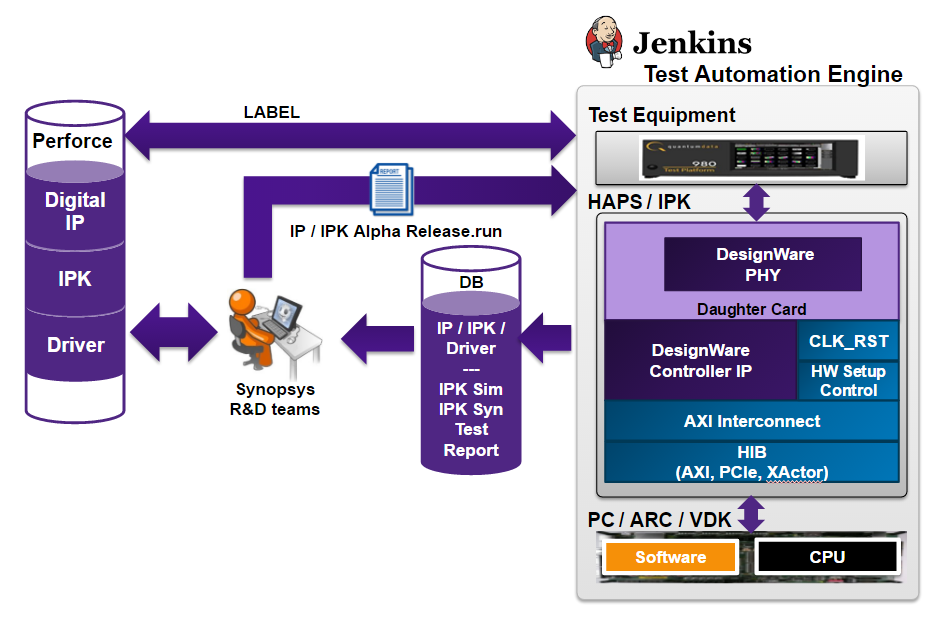
\includegraphics[width=1\textwidth]{ci_system_arch}}
      \caption{CI environment for Hardware Validation Context}
      \label{fig:ci_hw_context}
  \end{figure}
  
  
This architecture contains all the components used for a successful CI environment, as described in section \ref{sc:ciComponents}, being the object of test and analysis the multiple IP configurations, for the different communication interfaces, namely PCIe and ARC (see sections \ref{sc:pcie} and \ref{sc:arc}).

\subsection{Communication Interfaces}\label{sec:interfaces}

Here are succinctly described the HAPS platform and the different communication interfaces utilized as test objects by the IPK team. 

\subsubsection{HAPS}\label{sc:haps}

HAPS (High-performance ASIC Prototyping Systems) is an integrated and scalable hardware-software solution utilized by design and verification teams to improve their ASIC design schedules and avoid costly device re-spins\cite{HAPS}.

This prototyping solution consists of a collection of modular, easy-to-use products for ASIC and SoC prototyping that include HAPS hardware components supported by an integrated software tool flow for design planning, FPGA synthesis, and debug.

  \begin{figure}[H]
  \centering
      \makebox[\textwidth][c]{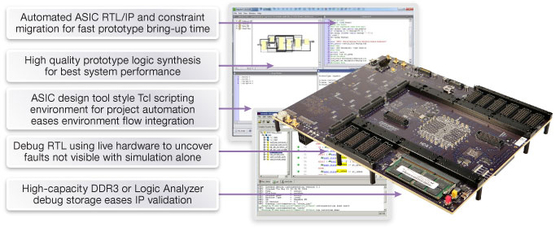
\includegraphics[width=0.5\textwidth]{haps}}
      \caption{HAPS®-Developer eXpress (HAPS-DX)}
      \label{fig:haps}
  \end{figure}

\subsubsection{ARC}\label{sc:arc}

Synopsys' DesignWare® ARC® Processors\cite{sns:ARC} are a family of 32-bit CPUs that SoC designers can optimize for a wide range of uses, from deeply embedded to high-performance host applications in a variety of market segments, such as Automotive and Industrial, Internet of Things or mobile. 

Designers can adapt their products by using configuration technology to tailor each ARC processor instance to meet specific performance, power and area requirements. These processors are also extendable, allowing designers to add their own custom instructions to increase performance.

  \begin{figure}[H]
  \centering
     \makebox[\textwidth][c]{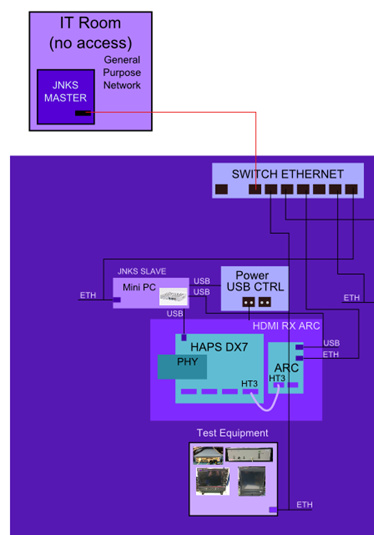
\includegraphics[width=0.5\textwidth]{arc}}
      \caption{ARC interface architecture}
     \label{fig:arc}
  \end{figure}


\subsubsection{PCIe}\label{sc:pcie}

PCI Express (Peripheral Component Interconnect Express), is a high-speed serial computer expansion bus standard, designed to replace the older bus standards\cite{wik:PCIE}\cite{sns:PCIE}.  Recent revisions of the PCIe standard provide hardware support for I/O virtualization.

The PCI Express electrical interface is also used in a variety of other standards, most notably in ExpressCard as a laptop expansion card interface, and in SATA Express as a computer storage interface.


 \begin{figure}[H]
  \centering
      \makebox[\textwidth][c]{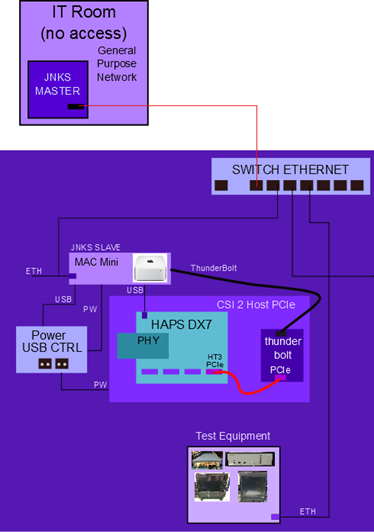
\includegraphics[width=0.5\textwidth]{pcie}}
      \caption{PCI Express (PCIe) interface architecture}
      \label{fig:pcie}
 \end{figure}

\subsection{CI-flow}\label{sc:workflow}

To better understand how the test automation for hardware/software validation works, the rundown of the process is described as follows:

\renewcommand{\labelenumii}{\theenumii}
\renewcommand{\theenumii}{\theenumi.\arabic{enumii}.}

\begin{enumerate}

\item The R\&D teams create an hardware image with a specific IP configuration to be deployed to the HAPS platform. At the same time, a firmware is packaged with its specific drivers to be deployed in the target interface, e.g. ARC and PCIe;

\item These files are committed to a VCS repository;

\item The Jenkins Master node receives notification of these changes and proceeds to run the associated Job. The Job is dispatched to the appropriate slave node, as seen in the figures \ref{fig:pcie} and \ref{fig:arc}, in a test automation rack that will trigger a set of sub-steps:

\begin{enumerate}
\item program the HAPS FPGA with the submitted hardware image;
\item boot the host interface and loads the firmware;
\item run a set of tests (IP compliance tests) from the test equipment and a log is generated;
\end{enumerate}

\item\label{failStep} The log is then parsed and a spreadsheet (detailed in section \ref{sec:spreadsheet}), containing all the relevant information is created. The spreadsheet is then validated by the R\&D teams.

\end{enumerate}

The last step of this flow is is faulted mainly by three dissatisfactory characteristics:

\begin{itemize}

\item The use of a spreadsheet file, which we detail its faults thoroughly in section~\ref{sec:spreadsheet}, that has no correlation with the Jenkins environment;

\item Jenkins default views of the IP projects do not display enough information to reach conclusions about the test results with ease;

\item Jenkins build views do not contain specific information about the configuration of the tested hardware, as seen in the figure \ref{fig:buildView}.

\end{itemize}

Ultimately, these are the points we want to correct in order to improve the last step, with this dissertation work.

\section{Solution Requirements}\label{sc:requirements}

For the display of the desired information in order for a better test result analysis, it was decided to implement a dashboard plugin as solution. Since dashboards allow stakeholders to monitor the contribution of the various elements in the organization. They allow the display of specific data points of the system in question, provided in a single "snapshot" \cite{dashboard}.

Presently, R\&D teams utilize an Excel spreadsheet created by its IP Prototyping Team, where most of the time the data is manually input with the test results obtained from a test compliance log. This method is a poor solution since it does not provide consistency between tests, nor automatic traceability among the different tested versions, as explained in section \ref{sec:spreadsheet}.

The dashboard plugin will serve as a project monitoring view where the R\&D teams can constantly observe the results of the hardware validation phase testing. The main features of the dashboard include:

\begin{itemize}
\item View customized to each development team;
\item Information of each test configuration;
\item Display of test results and build performance indicators (e.g. build average time of each configuration).
%\item Possibility of executing new tests with available alternative configurations.
\end{itemize}

\subsection{Project Views Alignment}\label{sc:projOrg}

The R\&D Jenkins environment is currently organized by different Views, each referencing a different project. As seen in the figure~\ref{fig:allViews}, a project View is very unidimensional, not displaying enough information.

Aware that each R\&D team can have more than one Project associated to it, this is one requirement we had in mind while creating our solution, as explained in section \ref{sc:implementationDesign}.

  \begin{figure}[H]
  \centering
      \makebox[\textwidth][c]{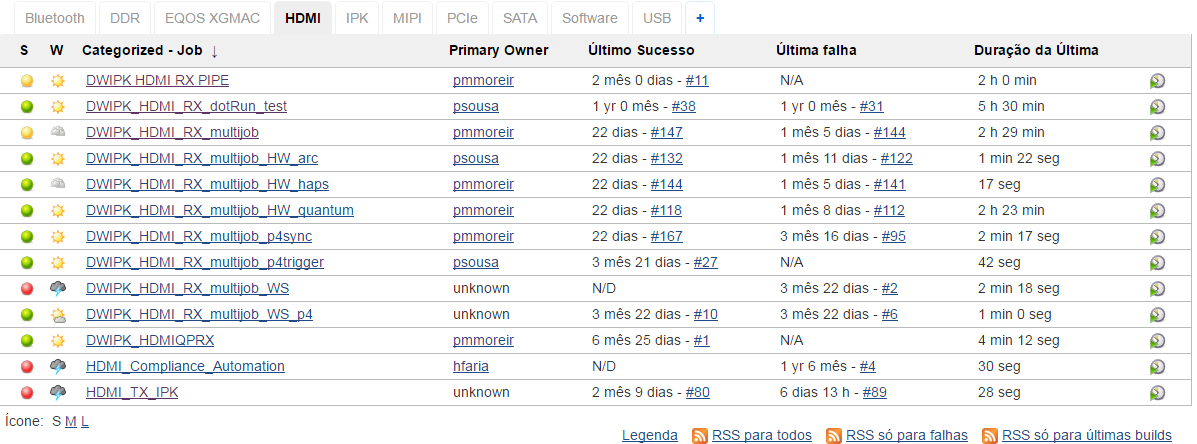
\includegraphics[width=1\textwidth]{allViews}}
      \caption{Project Views organized in the Jenkins system.}
      \label{fig:allViews}
  \end{figure}

\section{Project Build Spreadsheet}\label{sec:spreadsheet}

The IPK team uses an Excel Spreadsheet to track the overall status of each job with different test configurations, illustrated in figures \ref{fig:excel1} and \ref{fig:excel2}. 

  \begin{figure}[H]
  \centering
      \makebox[\textwidth][c]{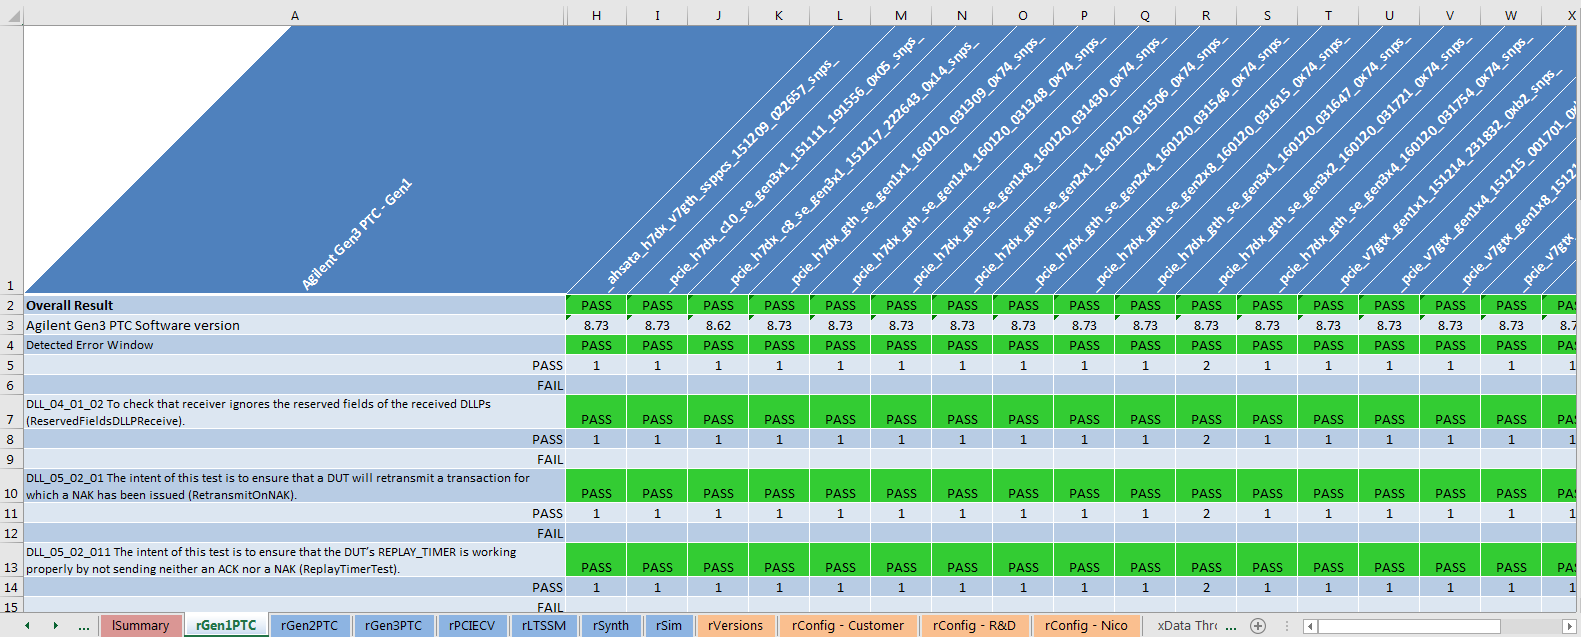
\includegraphics[width=1\textwidth]{excel1}}
      \caption{Hardware Test Summary Results}
      \label{fig:excel1}
  \end{figure}
  
Figure \ref{fig:excel1} depicts an example build run information in a PCIe interface. It is structured by the following elements:

\begin{itemize}
\item The labels in line 1 contain the project information, about the hardware build, namely the host interface, the PHY\cite{PHY} and top level hardware configurations, and date of the build;

\item The subsequent rows contain the test details, with the columns displaying information about the test result.
\end{itemize}
  
    \begin{figure}[H]
  \centering
      \makebox[\textwidth][c]{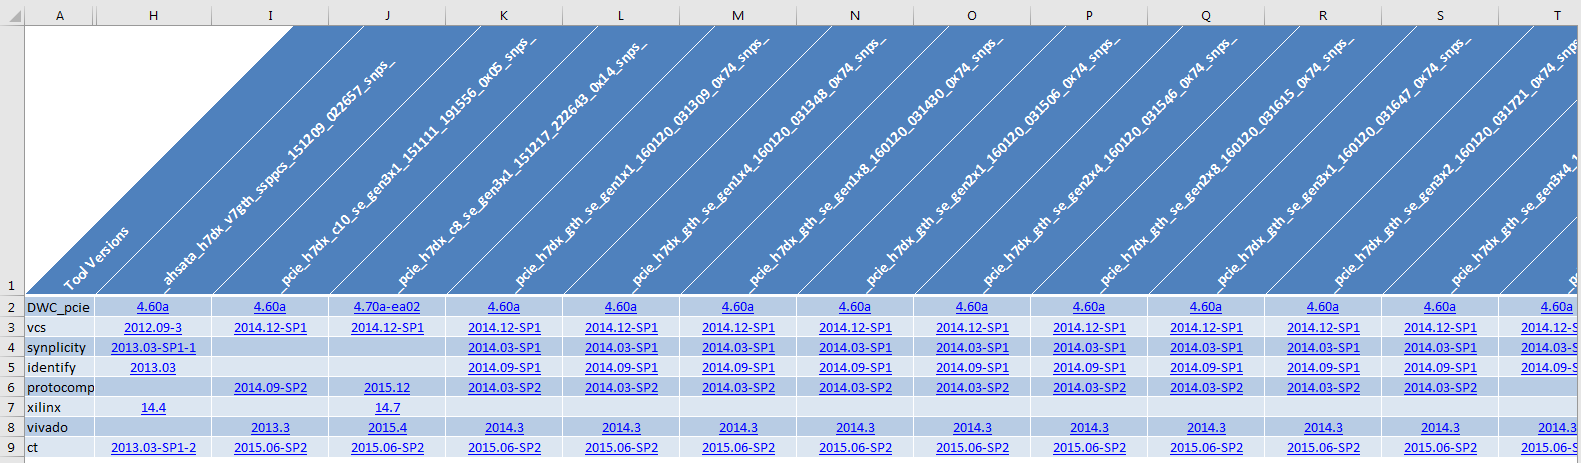
\includegraphics[width=1\textwidth]{excel2}}
      \caption{Different tools and controller Versions}
      \label{fig:excel2}
  \end{figure}

In figure \ref{fig:excel2} it is represented more information about the same build run, in a different sheet, showing the Controller Version in the first line, followed with the used tool versions for each configuration.

This exposes various problems, such as:

\begin{itemize}
\item \textbf{Traceability - } A new spreadsheet has to be created each time a new data-set of test results is created.
\item \textbf{Susceptible to Human Error - } If an error while populating the spreadsheet data is encountered, a manual fix is needed to correct it.
\item \textbf{Availability - } Every stakeholder in the process needs a copy of the spreadsheet for analysis.
\item \textbf{Difficulty to troubleshoot - } The need of correcting a failed test leads the user to search for it in the system.
\end{itemize}

A dashboard inside Jenkins will resolve this issues by aggregating the information in a single snapshot.

\section{Conclusion}\label{sec:conclusion_3}

Accuracy and speed need to be improved in the hardware validation process. Having a more centralized information access would greatly aid this improvement. 

Despite the fact that the organization of each project is well structured in Views, there is the need of a factor that facilitates its analysis, eliminating some of irrelevant information displayed.

The current solution is inefficient, with information disperse and more than required for the time being.

With this, it is safe to assume a View in form of a dashboard inside Jenkins is one optimal way to achieve this goal. Jenkins has a great API that allows access of its items inside its various Extension Points~\cite{jnks:extensionpoints}.

This will eliminate the issues of using a spreadsheet, since all the information is retrieved automatically from the Jenkins server in a reliable manner, and displayed available to every user inside the tool. It will make the validation process faster, concentrating the relevant information in a single view.